% =====================================================================
%  Шаблон методички «Линейная алгебра и геометрия для физиков»
%  Компиляция: XeLaTeX (Overleaf: Menu → Compiler → XeLaTeX).
%  Одна тема курса = одна глава (\chapter). Нумерация сквозная внутри главы:
%  Определение 1.2, Теорема 1.3, Лемма 1.4 — общий счётчик.
%  Всё, что выше строки «НАЧАЛО КОНТЕНТА», — общая преамбула: не менять
%  от главы к главе, чтобы методичка собиралась без правок.
% =====================================================================
\documentclass[12pt,a4paper]{report}

% ---------- Шрифты и язык ----------
\usepackage{fontspec}
\usepackage{polyglossia}
\setmainlanguage{russian}
\setotherlanguage{english}
\IfFontExistsTF{CMU Serif}{%
  \setmainfont{CMU Serif}\setsansfont{CMU Sans Serif}\setmonofont{CMU Typewriter Text}%
  \newfontfamily\cyrillicfont{CMU Serif}\newfontfamily\cyrillicfontsf{CMU Sans Serif}%
}{%
  \setmainfont{FreeSerif}\setsansfont{FreeSans}\setmonofont{DejaVu Sans Mono}%
  \newfontfamily\cyrillicfont{FreeSerif}\newfontfamily\cyrillicfontsf{FreeSans}%
}
\usepackage{amsmath,amssymb,amsthm,mathtools}
\usepackage{unicode-math}
\setmathfont{Latin Modern Math}

% ---------- Поля, заголовки, ссылки ----------
\usepackage[a4paper,margin=2.2cm,top=2cm,bottom=2.4cm]{geometry}
\usepackage{xcolor}
\usepackage{titlesec}
\usepackage{enumitem}
\usepackage[hidelinks]{hyperref}
\usepackage{qrcode}
\usepackage{graphicx}
\usepackage{tikz}
\usetikzlibrary{arrows.meta,calc,angles,quotes,decorations.pathmorphing,patterns,positioning}
\usepackage{pgfplots}\pgfplotsset{compat=1.18}
\usepackage[most]{tcolorbox}

% ---------- Цветовой код курса (един для всех глав и анимаций) ----------
\definecolor{cBase}{HTML}{1F5FBF}   % синий   — исходные векторы, базис, «до»
\definecolor{cImage}{HTML}{C8322A}  % красный — образы, результат действия, «после»
\definecolor{cEigen}{HTML}{1E8A4C}  % зелёный — собственные/инвариантные направления
\definecolor{cPhys}{HTML}{D97A00}   % оранжевый — физика: силы, токи, поля
\definecolor{cAux}{HTML}{7A7A7A}    % серый   — вспомогательные построения
\definecolor{cDef}{HTML}{1F5FBF}
\definecolor{cThm}{HTML}{6A3FA0}
\definecolor{cTrap}{HTML}{C8322A}
\colorlet{cDefBg}{cDef!6}
\colorlet{cThmBg}{cThm!6}
\colorlet{cPhysBg}{cPhys!8}

\tikzset{
  >={Stealth[length=2.6mm]},
  base/.style   ={->,very thick,cBase},
  img/.style    ={->,very thick,cImage},
  eigen/.style  ={->,very thick,cEigen},
  phys/.style   ={->,very thick,cPhys},
  aux/.style    ={cAux,dashed},
  grid lines/.style={cAux!35,thin},
}

% ---------- Заголовки глав ----------
\titleformat{\chapter}[display]
  {\normalfont\sffamily\bfseries\color{cBase}\raggedright}
  {\large Глава \thechapter}{0.4em}{\Huge}[\vspace{0.3em}{\color{cBase}\titlerule[1.2pt]}]
\titlespacing*{\chapter}{0pt}{-10pt}{18pt}
\titleformat{\section}{\normalfont\sffamily\Large\bfseries\color{cBase!85!black}}{\thesection}{0.6em}{}
\titleformat{\subsection}{\normalfont\sffamily\large\bfseries}{\thesubsection}{0.5em}{}

% ---------- Блоки: единый счётчик внутри главы ----------
\tcbset{
  lalgbox/.style={enhanced,sharp corners=south,arc=2mm,boxrule=0.6pt,
    left=3mm,right=3mm,top=1.5mm,bottom=1.5mm,
    fonttitle=\sffamily\bfseries,separator sign={.},description delimiters={(}{)}},
}
\newtcbtheorem[number within=chapter]{definition}{Определение}%
  {lalgbox,colback=cDefBg,colframe=cDef,coltitle=white}{def}
\newtcbtheorem[use counter from=definition]{theorem}{Теорема}%
  {lalgbox,colback=cThmBg,colframe=cThm,coltitle=white,fontupper=\itshape}{thm}
\newtcbtheorem[use counter from=definition]{lemma}{Лемма}%
  {lalgbox,colback=cThmBg,colframe=cThm!75,coltitle=white,fontupper=\itshape}{lem}
\newtcbtheorem[use counter from=definition]{corollary}{Следствие}%
  {lalgbox,colback=cThmBg,colframe=cThm!60,coltitle=white,fontupper=\itshape}{cor}

% Задача, с которой начинается тема: «есть проблема — чего не хватает?»
\newtcolorbox{problem}[1][]{enhanced,colback=cPhysBg,colframe=cPhys,
  boxrule=0pt,leftrule=3pt,sharp corners,left=3mm,
  title={\sffamily\bfseries Задача, с которой всё начинается#1},
  coltitle=cPhys!80!black,attach title to upper,after title={\par\smallskip}}
% Физическое приложение
\newtcolorbox{physics}[1]{enhanced,colback=cPhysBg,colframe=cPhys,
  boxrule=0.6pt,arc=2mm,fonttitle=\sffamily\bfseries,coltitle=white,
  title={Физика: #1}}
% Ловушка — тонкое место, на котором ловят на экзамене
\newtcolorbox{trap}{enhanced,colback=cTrap!5,colframe=cTrap,
  boxrule=0pt,leftrule=3pt,sharp corners,left=3mm,
  title={\sffamily\bfseries Осторожно},coltitle=cTrap,attach title to upper,
  after title={\enspace}}
% Вопрос, который возникает у студента по ходу чтения, — с ответом.
% Сюда идут реальные вопросы и ошибки, возникшие при разборе темы.
\newtcolorbox{studentq}[1]{enhanced,colback=cEigen!5,colframe=cEigen,
  boxrule=0pt,leftrule=3pt,sharp corners,left=3mm,
  title={\sffamily\bfseries Вопрос: #1},coltitle=cEigen!70!black,attach title to upper,
  after title={\par\smallskip}}
% Мост к следующей теме — держит единую линию повествования
\newtcolorbox{bridge}{enhanced,colback=cAux!8,colframe=cAux!8,arc=2mm,
  left=4mm,right=4mm,top=2mm,bottom=2mm,
  title={\sffamily\bfseries Что у нас есть и чего не хватает},
  coltitle=black,attach title to upper,after title={\par\smallskip}}

% ---------- Вёрстка без «висячих» строк ----------
% Ни одна строка абзаца не остаётся одна внизу или вверху страницы;
% страницы не растягиваются, если блок переехал на следующую.
\clubpenalty=10000 \widowpenalty=10000 \displaywidowpenalty=10000
\raggedbottom
% Цветные блоки (определения, теоремы, «Физика» и т. д.) не разрываются
% между страницами: они короткие, и разрыв мешает чтению.

% Доказательство — встроено в текст. Если доказательство помещается на странице,
% оно целиком переносится на новую страницу, когда на текущей не хватает места;
% разрывается только доказательство длиннее страницы.
\usepackage{environ,needspace}
\RenewEnviron{proof}[1][Доказательство]{%
  \par\smallskip
  \setbox0=\vbox{\hsize=\linewidth\noindent
    \textsf{\bfseries\color{cThm}#1.}\ \BODY\hfill$\blacksquare$}%
  \dimen0=\dimexpr\ht0+\dp0\relax
  \ifdim\dimen0<\dimexpr\textheight-2\baselineskip\relax
    \Needspace*{\dimen0}%
  \fi
  \noindent\textsf{\bfseries\color{cThm}#1.}\ \BODY\hfill$\blacksquare$\par\smallskip}

% Раскадровка анимации: кадры в ряд + QR на живую анимацию
%   \begin{frames}{подпись}{URL анимации} ... \frameitem{...} ... \end{frames}
\newcommand{\frameitem}[2][]{\begin{minipage}[t]{0.22\linewidth}\centering #2\\[-0.2em]
  {\footnotesize\sffamily #1}\end{minipage}\hfill}
\newenvironment{frames}[2]{\def\framescaption{#1}\def\framesurl{#2}%
  \begin{tcolorbox}[enhanced,colback=white,colframe=cAux!50,boxrule=0.5pt,arc=2mm,
    title={\sffamily\bfseries Анимация \hfill\normalfont\small смотреть по QR-коду или ссылке},
    coltitle=black,colbacktitle=cAux!12,sidebyside,lefthand ratio=0.86,
    sidebyside gap=3mm]\noindent}%
  {\tcblower\centering\qrcode[height=1.9cm]{\framesurl}\\[0.3em]
   {\tiny\href{\framesurl}{открыть}}\par
   \end{tcolorbox}\vspace{-0.6em}{\small\itshape\noindent\framescaption}\par\medskip}

% Задачи в конце блока
\newlist{exercises}{enumerate}{1}
\setlist[exercises]{label=\textsf{\bfseries\color{cBase}\thechapter.\arabic*.},left=0pt,itemsep=0.5em}
% Задачи: не меньше 5, из них 2–3 физические; вся нужная физика (кроме механики и МКТ)
% излагается прямо в условии — читатель-первокурсник её ещё не проходил.
\newcommand{\exhead}{\subsection*{Задачи}}
% Практика в конце главы: не меньше 5 вычислительных задач в стиле семинаров, ответы — в конце главы
\newlist{practice}{enumerate}{1}
\setlist[practice]{label=\textsf{\bfseries\color{cPhys}П\thechapter.\arabic*.},left=0pt,itemsep=0.5em}
\newcommand{\practicehead}{\section*{Практика}\addcontentsline{toc}{section}{Практика}
  {\small\itshape Задачи на счёт в стиле семинаров. Ответы — в конце главы.}\par\medskip}
\newlist{answers}{enumerate}{1}
\setlist[answers]{label=\textsf{\bfseries П\thechapter.\arabic*.},left=0pt,itemsep=0.2em,font=\small}
\newcommand{\answershead}{\subsection*{Ответы к практике}}

% Удобные обозначения
\newcommand{\R}{\mathbb{R}}
\newcommand{\C}{\mathbb{C}}
\DeclareMathOperator{\rk}{rk}
\DeclareMathOperator{\tr}{tr}
\renewcommand{\Im}{\operatorname{Im}}
\DeclareMathOperator{\Ker}{Ker}
\newcommand{\lin}[1]{\langle #1\rangle}

\setlength{\parindent}{1.2em}
\setlength{\parskip}{0.25em}

% =====================================================================
%  НАЧАЛО КОНТЕНТА. Ниже — образец главы: как выглядят все типы блоков.
% =====================================================================
\begin{document}

\begin{titlepage}\centering\sffamily
\vspace*{3cm}
{\Huge\bfseries\color{cBase} Линейная алгебра и геометрия\\[0.3em] для физиков\par}
\vspace{1em}{\Large методическое пособие для студентов-физиков\par}
\vspace{2.5cm}
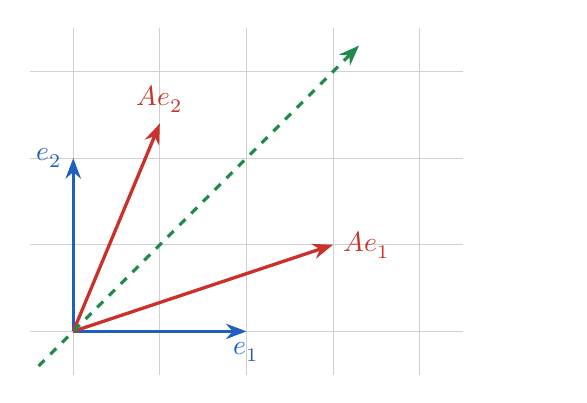
\begin{tikzpicture}[scale=1.1]
  \draw[grid lines] (-0.5,-0.5) grid (4.5,3.5);
  \draw[base] (0,0) -- (2,0) node[below] {$e_1$};
  \draw[base] (0,0) -- (0,2) node[left] {$e_2$};
  \draw[img] (0,0) -- (3,1) node[right] {$Ae_1$};
  \draw[img] (0,0) -- (1,2.4) node[above] {$Ae_2$};
  \draw[eigen,dashed] (-0.4,-0.4) -- (3.3,3.3) node[right] {собственное направление};
\end{tikzpicture}
\vfill
\begin{tabular}{rl}
\textcolor{cBase}{\rule{1.2em}{0.6em}} & исходные векторы, базис\\
\textcolor{cImage}{\rule{1.2em}{0.6em}} & образы, результат действия\\
\textcolor{cEigen}{\rule{1.2em}{0.6em}} & собственные и инвариантные направления\\
\textcolor{cPhys}{\rule{1.2em}{0.6em}} & физические величины
\end{tabular}
\vspace{1cm}
\end{titlepage}

\tableofcontents

% ---------------------------------------------------------------------
\chapter{Линейная зависимость}
% ---------------------------------------------------------------------

\begin{problem}
К телу приложены три силы, и оно покоится. Мы знаем две из них. Можно ли
по ним однозначно восстановить третью? А если сил десять, а тело — в плоскости?
Сколько среди них на самом деле «независимых», и что это слово вообще значит?
\end{problem}

Условие равновесия записывается одной строкой: $\vec F_1+\vec F_2+\vec F_3=0$.
Это сумма векторов с коэффициентами $1,1,1$, равная нулю. Такие суммы
встречаются в физике постоянно — суперпозиция полей, правила Кирхгофа, —
поэтому дадим им имя.

\begin{figure}[h]\centering
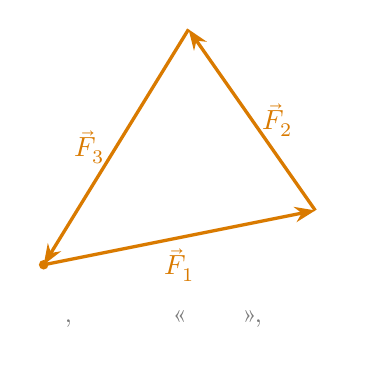
\begin{tikzpicture}[scale=1.15]
  \draw[phys] (0,0) -- (3,0.6) node[midway,below] {$\vec F_1$};
  \draw[phys] (3,0.6) -- (1.6,2.6) node[midway,right] {$\vec F_2$};
  \draw[phys] (1.6,2.6) -- (0,0) node[midway,left] {$\vec F_3$};
  \fill[cPhys] (0,0) circle (1.5pt);
  \node[cAux,font=\small] at (1.6,-0.6) {силы, перенесённые «цепочкой», замыкаются};
\end{tikzpicture}
\caption{Три силы в равновесии образуют замкнутый треугольник:
каждая выражается через две другие.}
\end{figure}

\begin{definition}{Линейная зависимость}{lindep}
Система векторов $a_1,\dots,a_k$ называется \emph{линейно зависимой},
если существуют числа $\alpha_1,\dots,\alpha_k$, \textbf{не все равные нулю},
такие что $\alpha_1a_1+\dots+\alpha_ka_k=0$. В противном случае система
\emph{линейно независима}: равенство нулю линейной комбинации возможно
только при всех нулевых коэффициентах.
\end{definition}

\begin{studentq}{почему бы не потребовать, чтобы все коэффициенты были ненулевыми?}
Тогда система $0,\,a$ (нулевой вектор и любой другой) оказалась бы «независимой»,
хотя нулевой вектор заведомо ни к чему не привязан и выражается через что угодно.
Определение должно ловить \emph{любую} лишнюю связь, а для этого достаточно
одного ненулевого коэффициента.
\end{studentq}

\begin{trap}
Не «все коэффициенты ненулевые», а «хотя бы один ненулевой».
Система $0,\,a$ зависима: $1\cdot 0+0\cdot a=0$.
\end{trap}

Определение говорит о равенстве нулю, а в задаче нас интересовало,
выражается ли одна сила через остальные. Это одно и то же:

\begin{lemma}{}{express}
Система из $k\ge2$ векторов линейно зависима тогда и только тогда,
когда хотя бы один из них выражается линейной комбинацией остальных.
\end{lemma}
\begin{proof}
Пусть $\sum\alpha_ia_i=0$ и, скажем, $\alpha_1\neq0$. Делим на $\alpha_1$:
$a_1=-\sum_{i\ge2}(\alpha_i/\alpha_1)\,a_i$. Обратно, если
$a_1=\sum_{i\ge2}\beta_ia_i$, то $1\cdot a_1-\sum\beta_ia_i=0$ — нетривиальная
комбинация, ведь коэффициент при $a_1$ равен $1$.
\end{proof}

\begin{physics}{первое правило Кирхгофа}
Токи, втекающие в узел, удовлетворяют $I_1+I_2+\dots+I_n=0$. Поэтому
уравнения для токов всех узлов цепи линейно зависимы: одно из них
всегда следует из остальных. Отсюда правило «уравнений на одно меньше,
чем узлов».
\end{physics}

\begin{frames}{Сдвиг $A=\begin{psmallmatrix}1&1\\0&1\end{psmallmatrix}$ при $t=0\to1$:
синий квадрат базиса превращается в красный параллелограмм, а ось $x$
(зелёная) остаётся на месте — это собственное направление.}{https://smbym.github.io/linal-nsu-ff/anim/01-shear.gif}
\foreach \t/\lab in {0/{$t=0$},0.33/{$t=\tfrac13$},0.67/{$t=\tfrac23$},1/{$t=1$}}{%
\frameitem[\lab]{\begin{tikzpicture}[scale=0.9]
  \draw[grid lines] (-0.2,-0.2) grid (2.2,1.2);
  \draw[eigen] (0,0) -- (1.9,0);
  \fill[cBase!15] (0,0) rectangle (1,1);
  \fill[cImage!25,opacity=0.8] (0,0) -- (1,0) -- (1+\t,1) -- (\t,1) -- cycle;
  \draw[img] (0,0) -- (\t,1);
\end{tikzpicture}}}
\end{frames}

\exhead
\begin{exercises}
\item \textit{(Физика.)} Напряжённость электростатического поля точечного заряда $q$
  в точке $P$ — это вектор, направленный вдоль прямой, соединяющей заряд и $P$
  (от заряда при $q>0$), по модулю равный $k|q|/r^2$, где $r$ — расстояние до заряда.
  Поля нескольких зарядов складываются как векторы (принцип суперпозиции).
  Три заряда создают в точке $P$ поля $\vec E_1,\vec E_2,\vec E_3$, причём
  суммарное поле в $P$ равно нулю. Докажите, что система $\vec E_1,\vec E_2,\vec E_3$
  линейно зависима, и выразите $\vec E_3$ через остальные.
\item Докажите, что подсистема линейно независимой системы линейно независима.
\item Докажите, что система, содержащая нулевой вектор или два пропорциональных
  вектора, линейно зависима.
\item \textit{(Физика.)} \emph{Первое правило Кирхгофа:} в узле электрической цепи
  заряд не накапливается, поэтому сумма токов, втекающих в узел, равна сумме вытекающих.
  Два узла $A$ и $B$ соединены тремя проводами; токи $I_1,I_2,I_3$ считаем
  положительными, если они текут от $A$ к $B$. Запишите правило Кирхгофа для каждого
  узла и докажите, что эти два уравнения линейно зависимы. Сколько из них независимых?
\item \textit{(Физика.)} Материальная точка покоится под действием сил
  $\vec F_1,\dots,\vec F_n$ (по второму закону Ньютона при нулевом ускорении
  векторная сумма сил равна нулю). Докажите, что система сил линейно зависима,
  и укажите, какая сила выражается через остальные.
\end{exercises}


\practicehead
\begin{practice}
\item Выясните, линейно зависима ли система $(1,2,3)$, $(4,5,6)$, $(7,8,9)$.
  Если да — найдите нетривиальную линейную комбинацию, равную нулю.
\item Выясните, линейно зависима ли система $(1,0,1)$, $(0,1,1)$, $(1,1,0)$.
\item Найдите все пары $(\alpha,\beta)$, при которых $\alpha(1,2)+\beta(3,6)=0$.
\item При каких $\lambda$ векторы $(1,1,\lambda)$, $(1,\lambda,1)$, $(\lambda,1,1)$ линейно зависимы?
\item На тело действует сила $\vec F=(5,1)$. Разложите её по направлениям двух тросов
  $\vec f_1=(1,1)$ и $\vec f_2=(2,-1)$: найдите $\alpha,\beta$, при которых $\vec F=\alpha\vec f_1+\beta\vec f_2$.
\end{practice}

\answershead
\begin{answers}
\item Зависима: $(1,2,3)-2\,(4,5,6)+(7,8,9)=0$.
\item Независима.
\item $\alpha=-3t$, $\beta=t$, $t\in\R$.
\item $\lambda=1$ и $\lambda=-2$.
\item $\alpha=7/3$, $\beta=4/3$.
\end{answers}

\begin{bridge}
Мы умеем узнавать, выражается ли вектор через другие. Но в задаче
о десяти силах на плоскости нас интересует, \emph{сколько} независимых
векторов в ней может быть вообще — и почему это число не зависит
от того, какие именно векторы мы выбрали. Для ответа нужна лемма о замене,
и с неё начинается следующий раздел.
\end{bridge}

\end{document}
